\documentclass[11pt]{article}
\usepackage{amsmath, amssymb, geometry, tikz}
\usepackage{fancyhdr}
\geometry{a4paper, margin=1in}

\pagestyle{fancy}
\fancyhf{} % Clears all default header and footer fields
\fancyhead[R]{sujeet.banerjee@gmail.com
\\
sujeet.banerjee.pofessional@gmail.com} % Sets the right header
\fancyhead[L]{Agentic AI Bootcamp}
\fancyfoot[R]{\thepage} % Keeps the page number at the bottom center
\fancyfoot[L]{Vectors, Dot, Cosine}
\renewcommand{\headrulewidth}{0.4pt} % Adds a decorative line under the header (optional)
\renewcommand{\footrulewidth}{0.4pt}


\title{\textbf{Practice Sheet \& Notes:\\ 2D Vectors, Dot-product and Cosine Similarity}}
\author{}
\date{}

\begin{document}
\maketitle

\section*{Study Notes}

\subsection*{1. Specifying 2D Points (Latitude and Longitude)}
In a 2D Cartesian coordinate system, a point is specified by a pair of values $(x, y)$. For geographical or spatial contexts, the X-axis typically represents \textbf{Longitude} (East-West position), and the Y-axis represents \textbf{Latitude} (North-South position). The point $\mathbf{O}$ represents the Origin, or $(0,0)$.

\textbf{Example Graph:} Let us plot three points: $A(2, 3)$, $B(-2, 1)$, and $C(3, -2)$.

\begin{center}
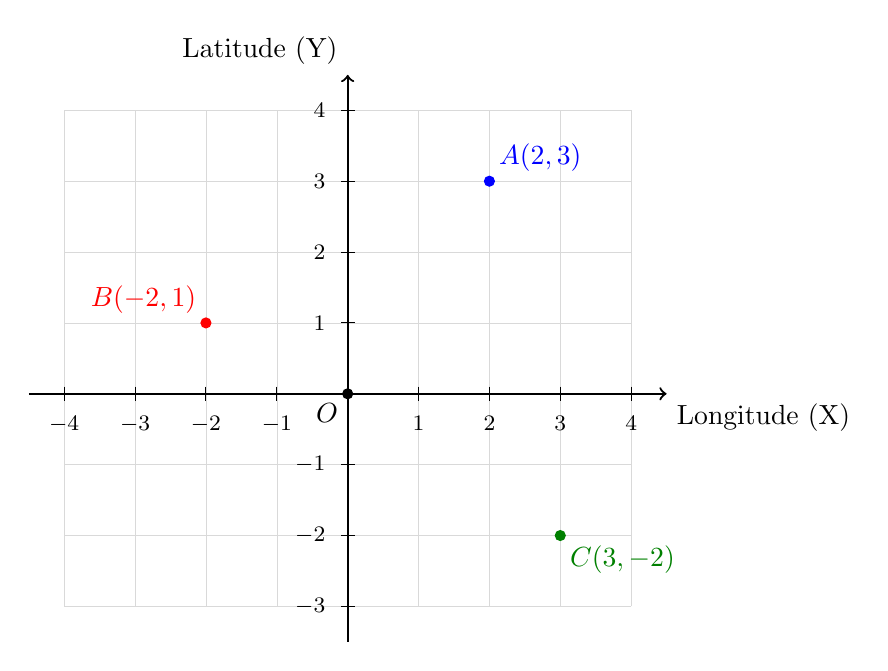
\begin{tikzpicture}[scale=0.9]
    % Grid
    \draw[step=1cm,gray!30,very thin] (-4,-3) grid (4,4);
    % Axes
    \draw[thick,->] (-4.5,0) -- (4.5,0) node[anchor=north west] {Longitude (X)};
    \draw[thick,->] (0,-3.5) -- (0,4.5) node[anchor=south east] {Latitude (Y)};
    
    % Points
    \filldraw[blue] (2,3) circle (2pt) node[anchor=south west] {$A(2,3)$};
    \filldraw[red] (-2,1) circle (2pt) node[anchor=south east] {$B(-2,1)$};
    \filldraw[green!50!black] (3,-2) circle (2pt) node[anchor=north west] {$C(3,-2)$};
    \filldraw[black!10!black] (0,0) circle (2pt) node[anchor=north east ] {$O$};
    
    % Ticks
    \foreach \x in {-4,-3,-2,-1,1,2,3,4} \draw (\x,0.1) -- (\x,-0.1) node[below=2pt] {\footnotesize $\x$};
    \foreach \y in {-3,-2,-1,1,2,3,4} \draw (0.1,\y) -- (-0.1,\y) node[left=2pt] {\footnotesize $\y$};
\end{tikzpicture}
\end{center}

\subsection*{2. Euclidean Distance Between Two Points}
The Euclidean distance $d$ between two points $P_1(x_1, y_1)$ and $P_2(x_2, y_2)$ is given by the formula:
\[ d = \sqrt{(x_2 - x_1)^2 + (y_2 - y_1)^2} \]

\textbf{Example Calculation:} Find the distance between $A(2,3)$ and $B(-2,1)$.
\[ d(A,B) = \sqrt{(-2 - 2)^2 + (1 - 3)^2} = \sqrt{(-4)^2 + (-2)^2} = \sqrt{16 + 4} = \sqrt{20} = 2\sqrt{5} \approx 4.47 \]

\subsection*{3. Norm (Magnitude) of Position Vectors}
When a point $P(x,y)$ is treated as a position vector $\vec{P}$ starting from the origin $(0,0)$, its \textbf{norm} (or length) is denoted by $\|\vec{P}\|$.
\[ \|\vec{P}\| = \sqrt{x^2 + y^2} \]

\textbf{Example Calculation:} Find the norm of the position vector for $A(2,3)$.
\[ \|\vec{A}\| = \sqrt{2^2 + 3^2} = \sqrt{4 + 9} = \sqrt{13} \approx 3.61 \]

\begin{center}
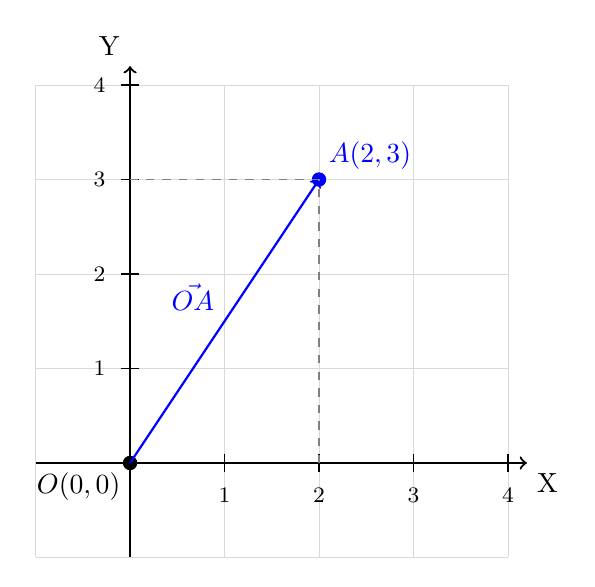
\begin{tikzpicture}[scale=1.2]
    % Grid
    \draw[step=1cm,gray!30,very thin] (-1,-1) grid (4,4);
    
    % Axes
    \draw[thick,->] (-1,0) -- (4.2,0) node[anchor=north west] {X};
    \draw[thick,->] (0,-1) -- (0,4.2) node[anchor=south east] {Y};
    
    % Ticks
    \foreach \x in {1,2,3,4} \draw (\x,0.1) -- (\x,-0.1) node[below=2pt] {\footnotesize $\x$};
    \foreach \y in {1,2,3,4} \draw (0.1,\y) -- (-0.1,\y) node[left=2pt] {\footnotesize $\y$};
    
    % Origin O
    \filldraw[black] (0,0) circle (2pt) node[anchor=north east] {$O(0,0)$};
    
    % Point A
    \filldraw[blue] (2,3) circle (2pt) node[anchor=south west] {$A(2,3)$};
    
    % Position Vector OA
    \draw[thick, ->, blue] (0,0) -- (2,3) node[midway, anchor=south east] {$\vec{OA}$};
    
    % Dashed lines to show coordinates
    \draw[dashed, gray] (2,0) -- (2,3) -- (0,3);
\end{tikzpicture}
\end{center}
The length of the point vector $\vec{OA}$ is $\approx 3.61$

\subsection*{4. Dot Product of Position Vectors}
The dot product of two position vectors $\vec{U} = \langle x_1, y_1 \rangle$ and $\vec{V} = \langle x_2, y_2 \rangle$ is a scalar value calculated as:
\[ \vec{U} \cdot \vec{V} = (x_1 \times x_2) + (y_1 \times y_2) \]

\textbf{Example Calculation:} Find the dot product of $\vec{A} = \langle 2, 3 \rangle$ and $\vec{B} = \langle -2, 1 \rangle$.
\[ \vec{A} \cdot \vec{B} = (2 \times -2) + (3 \times 1) = -4 + 3 = -1 \]

\subsection*{5. Cosine Similarity Score}
The cosine similarity score measures how aligned two vectors are, independent of their magnitude. It represents the cosine of the angle $\theta$ between the points.
\[ \text{Cosine Similarity} = \cos(\theta) = \frac{\vec{U} \cdot \vec{V}}{\|\vec{U}\| \|\vec{V}\|} \]
\textbf{Note:} The similarity values have a cap (maximum) value of $1$. A value of $1$ indicates a perfectly overlapping orientation (the vectors point in the exact same direction). A value of $0$ means the vectors are wide apart at exactly $90^\circ$ (orthogonal). Negative values indicate they point in opposing directions.

\begin{center}
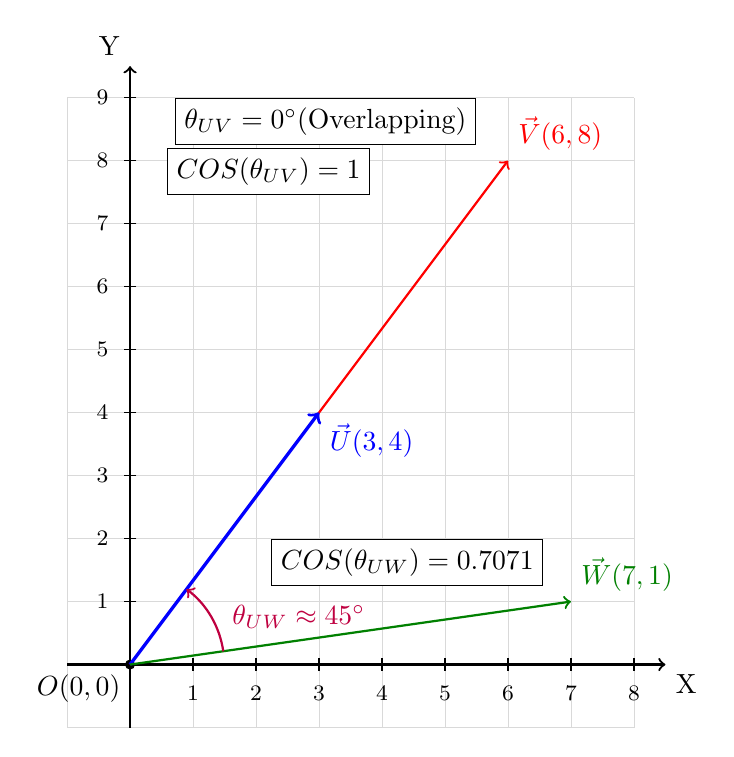
\begin{tikzpicture}[scale=0.8]
    % Grid
    \draw[step=1cm,gray!30,very thin] (-1,-1) grid (8,9);
    
    % Axes
    \draw[thick,->] (-1,0) -- (8.5,0) node[anchor=north west] {X};
    \draw[thick,->] (0,-1) -- (0,9.5) node[anchor=south east] {Y};
    
    % Ticks
    \foreach \x in {1,2,3,4,5,6,7,8} \draw (\x,0.1) -- (\x,-0.1) node[below=2pt] {\footnotesize $\x$};
    \foreach \y in {1,2,3,4,5,6,7,8,9} \draw (0.1,\y) -- (-0.1,\y) node[left=2pt] {\footnotesize $\y$};
    
    % Origin O
    \filldraw[black] (0,0) circle (2pt) node[anchor=north east] {$O(0,0)$};
    
    % Draw Vector V (drawn first so U can overlay on it)
    \draw[thick, ->, red] (0,0) -- (6,8) node[anchor=south west] {$\vec{V}(6,8)$};
    
    % Draw Vector U (overlaps V)
    \draw[very thick, ->, blue] (0,0) -- (3,4) node[anchor=north west] {$\vec{U}(3,4)$};
    
    % Draw Vector W
    \draw[thick, ->, green!50!black] (0,0) -- (7,1) node[anchor=south west] {$\vec{W}(7,1)$};
    
    % Angle between U and W
    % W is at ~8.13 degrees, U is at ~53.13 degrees
    \draw[thick, ->, purple] (1.48, 0.21) arc (8.13:53.13:1.5) node[midway, right=4pt] {$\theta_{UW} \approx 45^{\circ} $};
    \node[fill=white, draw=black, thin, anchor=north] at (4.40, 2.0) {$COS(\theta_{UW}) = 0.7071 $};
    
    % Note indicating the overlapping vectors and their 0 degree angle
    \node[fill=white, draw=black, thin, anchor=north] at (3.1, 9) {$\theta_{UV} = 0^\circ$ 
    \newline 
    (Overlapping) };
    
    % Note indicating the overlapping vectors and their 0 degree angle
    \node[fill=white, draw=black, thin, anchor=north] at (2.2, 8.2) {$COS(\theta_{UV}) = 1 $};
    
\end{tikzpicture}
\end{center}
\\

\textbf{Example Calculation 1 (Overlapping vectors):} \\
Let $\vec{U} = \langle 3, 4 \rangle$ and $\vec{V} = \langle 6, 8 \rangle$.
\[ \vec{U} \cdot \vec{V} = (3)(6) + (4)(8) = 18 + 32 = 50 \]
\[ \|\vec{U}\| = \sqrt{3^2+4^2}=5, \quad \|\vec{V}\| = \sqrt{6^2+8^2}=10 \]
\[ \text{COSINE}(\vec{U},\vec{V}) = \frac{50}{5 \times 10} = \frac{50}{50} = 1 \]
\textit{Result:} Cosine score = 1 (Perfectly overlapping orientation; or highly \textbf{similar}).
\\ 

\textbf{Example Calculation 2 (dissimilar vectors):} \\
Let $\vec{U} = \langle 3, 4 \rangle$ and $\vec{W} = \langle 7, 1 \rangle$.
\[ \vec{U} \cdot \vec{W} = (3)(7) + (4)(1) = 21 + 4 = 25 \]
\[ \|\vec{U}\| = \sqrt{3^2+4^2}=5, \quad \|\vec{W}\| = \sqrt{7^2+1^2}= \sqrt{50} \approx 7.1 \]
\[ \text{COSINE}(\vec{U},\vec{W}) = \frac{25}{5 \times 7.1} = \frac{50}{35.5} = 0.7071 \]
\textit{Result:} Cosine score = 0.7071 (\textbf{slightly dissimilar}).
\\

\textbf{Example Calculation 3 (Orthogonal vectors):} \\
Let $\vec{X} = \langle 1, 0 \rangle$ and $\vec{Y} = \langle 0, 1 \rangle$.
\[ \vec{X} \cdot \vec{Y} = (1)(0) + (0)(1) = 0 \]
\[ \text{COSINE}(\vec{X},\vec{Y}) = \frac{0}{1 \times 1} = 0 \]
\textit{Result:} Cosine score = 0 (Wide apart, $90^\circ$ separation; or highly \textbf{dissimilar}).

\newpage
\section*{Practice Questions}

\textbf{Q1: Specifying Coordinates}\\
Let three locations on a map be given by their (Longitude, Latitude) coordinates: $P(3, 4)$, $Q(-1, 2)$, and $R(4, -3)$.
\begin{enumerate}
    \item[(a)] Draw a Cartesian plane, label the axes appropriately (Longitude / Latitude), and plot points $P$, $Q$, and $R$.
    \item[(b)] Express $P$, $Q$, and $R$ as position vectors originating from $(0,0)$.
\end{enumerate}

\textbf{Q2: Euclidean Distance}\\
Using the points from Q1:
\begin{enumerate}
    \item[(a)] Calculate the straight-line Euclidean distance between $P$ and $Q$.
    \item[(b)] Calculate the straight-line Euclidean distance between $Q$ and $R$.
\end{enumerate}

\textbf{Q3: Norm Computations}\\
Calculate the norm (magnitude) of the following position vectors:
\begin{enumerate}
    \item[(a)] $\|\vec{P}\|$
    \item[(b)] $\|\vec{Q}\|$
    \item[(c)] $\|\vec{R}\|$
\end{enumerate}

\textbf{Q4: Dot Products}\\
Compute the dot product for the following pairs of position vectors:
\begin{enumerate}
    \item[(a)] $\vec{P} \cdot \vec{Q}$
    \item[(b)] $\vec{Q} \cdot \vec{R}$
    \item[(c)] $\vec{P} \cdot \vec{R}$
\end{enumerate}

\textbf{Q5: Cosine Similarity}\\
Calculate the cosine similarity score between the following pairs. (Leave answers in exact fraction/radical form if necessary).
\begin{enumerate}
    \item[(a)] $\vec{P}$ and $\vec{Q}$
    \item[(b)] $\vec{Q}$ and $\vec{R}$
\end{enumerate}

\textbf{Q6: Orthogonality (90-Degree Separation)}\\
A new point $S$ has coordinates $(x, 6)$.
\begin{enumerate}
    \item[(a)] Write the position vector for $S$ in terms of $x$.
    \item[(b)] Find the value of $x$ such that $\vec{S}$ is exactly $90^\circ$ apart from $\vec{P}(3, 4)$ (i.e., their cosine similarity score is $0$).
\end{enumerate}

\textbf{Q7: Overlapping Orientations}\\
Consider a point $T(9, 12)$.
\begin{enumerate}
    \item[(a)] Calculate the cosine similarity score between $\vec{P}(3, 4)$ and $\vec{T}$.
    \item[(b)] Interpret the physical meaning of this score in terms of their orientation.
\end{enumerate}

\textbf{Q8: Geometric Application}\\
Consider the vectors $\vec{M} = \langle 5, 2 \rangle$ and $\vec{N} = \langle -2, 5 \rangle$.
\begin{enumerate}
    \item[(a)] Calculate their dot product and the cosine similarity score.
    \item[(b)] Based on the cosine similarity score, what is the exact angle between $\vec{M}$ and $\vec{N}$?
    \item[(c)] Find the Euclidean distance between points $M$ and $N$.
    \item[(d)] Verify that the triangle formed by the Origin $(0,0)$, $M$, and $N$ satisfies the Pythagorean theorem ($OM^2 + ON^2 = MN^2$).
\end{enumerate}

\end{document}
